\chapter{Primary Decomposition}

Let $R$ be a nonzero commutative ring with identity.

\begin{discussion}
    UFD's have prime factorization. In fact, it is ``if and only if''. \par 
    Aternative versions for non-UFD's.
    \begin{enumerate}
        \item irreducible factorizations: 
            \[
                \begin{array}{llll}
                    \text{\underline{Pros}} &&& \text{\underline{Cons}} \\
                    \text{familiar} &&& \text{don't necessarily exist} 
                \end{array}.
            \]
        \item 
            primary decompositions:
            \[
                \begin{array}{llll}
                    \text{\underline{Pros}} &&& \text{\underline{Cons}} \\
                    \text{exist, e.g., if $R$ is noetherian,} &&& \text{replace factorizations of elements} \\
                    \text{there exists more generators } &&& \text{with intersections of nice ideal} \\
                    \text{than just for principal ideal}
                \end{array}.
            \]
    \end{enumerate}
\end{discussion}

\begin{theorem}
    Let $R$ be a noetherian integral domain and $a \in R \setminus \{R^{\times} \cup 0\}$.
    \begin{enumerate}
        \item $a$ has an irreducible factor in $R$.
        \item There exist irreducible $b_1,\cdots,b_n \in R$ such that $a = b_1 \cdots b_n$.
    \end{enumerate}
\end{theorem}

\begin{proof}
    \begin{enumerate}
        \item Let $\Sigma = \{\langle b \rangle \neq R : b \mid a\}$. Since $\langle a \rangle \in \Sigma$, $\Sigma \neq \emptyset$. Since $R$ is noetherian, $\Sigma$ has a maximal element, say $\langle b \rangle$. Claim. $\langle b \rangle$ is irreducible. Note $b \neq 0$ since $a \neq 0$ and $b \mid a$, and $b \not \in R^{\times}$ since $\langle b \rangle \neq R$. Suppose $b = cd$ for some $c,d \in R$. Since $c \mid b \mid a$, we have $c \mid a$. Also, since $c \not \in R^{\times}$, $\langle c \rangle \in \Sigma$. Since $\langle b \rangle \subseteq \langle c \rangle \subseteq R$, $\langle b \rangle$ is maximal in $\Sigma$, we have $\langle cd \rangle = \langle b \rangle = \langle c \rangle$ or $\langle c \rangle = R$. Since $R$ is an integral domain, $d \in R^{\times}$ or $c \in R^{\times}$.
        \item If $a$ is irreducible, then done. Else there exists $b_1 \in R$ irreducible such that $b_1 \mid a$ and $a = b_1a_1$ for some $a_1 \in R$. If $a_1$ is irreducible, then done. Else there exists irreducible $b_2 \in R$ such that $b_2 \mid a_1$ and $a_1 = b_2a_2$ for some $a_2 \in R$. If $a_2$ is irreducible, then done and we have $\langle a \rangle \subsetneq \langle a_1 \rangle \subsetneq \langle a_2 \rangle$. By the ascending chain condition, the process will terminate in finite number of steps. \qedhere
    \end{enumerate}
\end{proof}

\begin{example}
    \begin{enumerate}
        \item 
            Let $k$ be a field and $A = k[X^{\bbR_{\geq 0}}] := \{\sum_{i \in \bbR_{\geq 0}}^{\text{finite}}a_iX^{i} \mid a_i \in k\}$. Let $\ffm = \langle X^{\bbR_{>0}} \rangle \lneq A$. Then $\ffm \in \operatorname{m-Spec}(R)$ and $A/\ffm \cong k$. Let $R = A_\ffm$. Since $X$ has no irreducible factors in $R$, $X$ has no irreducible factorization. Let $\epsilon > 0$ and $f \in R \setminus \{0\}$. Then $R \setminus \{R^{\times} \cup 0\} \ni X^{\epsilon} \cdot f = X^{\frac{\epsilon}{2}} \cdot X^{\frac{\epsilon}{2}} \cdot f$. So $X^{\epsilon}f$ is not irreducible. Thus, $R$ has no irreducible elements.
        \item 
            In $\bbZ_6$, we have $3^{2} = 3$, $2^{2} = 4$, $2^{3} = 2$.
    \end{enumerate}
\end{example}

\begin{definition}
    If $R$ satisfies the conclusion of Theorem 4.2(b), then $R$ is \emph {atomic}.
\end{definition}

\begin{lemma}[Nakayama's Lemma]
    Let $I,J \leq R$ such that $I \subseteq \operatorname{Jac}(R)$ and $J$ is finitely generated. If $J = IJ$, then $J = 0$.
\end{lemma}

\begin{proof}
    Let $n$ be the minimum number of generators of $J$. Suppose $n \geq 2$. Since $J$ is finitely generated, $IJ = J = \langle x_1,\cdots,x_n \rangle$. Then $x_n \in IJ$ and so $x_n = \sum_{i=1}^{n}a_ix_i$ for some $a_1,\cdots,a_n \in I$. Hence $x_n(1-a_n) = \sum_{i=1}^{n}a_ix_i$. Since $a_n \in I \in \operatorname{Jac}(R)$, $1-a_n \in R^{\times}$ by Proposition 1.29. So $x_n \in \langle X_1,\cdots,X_{n-1} \rangle$, contradicting minimality of $n$. Hence $n = 1$ or $0$. If $n = 1$, similarly, we have $x_1(1-a_1) = 0$ for some $a_1 \in I$ with $1-a_1 \in R^{\times}$, so $x_1 = 0$, a contradiction. Thus, $n = 0$.
\end{proof}

\begin{lemma}
    Let $(R,\ffm)$ be local and $0 \neq b = cd$ with $b,c,d \in R$ such that $\langle b \rangle = \langle c \rangle$. Then $d \in R^{\times}$.
\end{lemma}

\begin{proof}
    Since $b = cd$ and $\langle b \rangle = \langle c \rangle$, we have $\langle c \rangle = \langle b \rangle = \langle cd \rangle = \langle d \rangle \langle c \rangle$. Suppose $d \not \in R^{\times}$. Then $\langle d \rangle \subseteq \ffm = \operatorname{Jac}(R)$. So by Lemma 4.5, $c = 0$. Hence $b = cd = 0$, a contradiction. Thus, $d \in R^{\times}$.
\end{proof}

\begin{theorem}
    Let $(R,\ffm)$ be local and noetherian. Let $a \in R \setminus \{R^{\times} \cup 0\}$. 
    \begin{enumerate}
        \item $a$ has an irreducible factor in $R$.
        \item $a = b_1 \cdots b_n$ for some irreducible elements $b_1,\cdots,b_n \in R$.
    \end{enumerate}
\end{theorem}

\begin{proof}
    Similar to the proof of Theorem 4.2.
\end{proof}

\begin{discussion}
    Let $R$ be noetherian (local or a domain) and $a \in R \setminus \{R^{\times} \cup 0\}$ with irreducible factorization $a = b_1 \cdots b_n$. Then $\operatorname{V}(a) = \operatorname{V}(b_1 \cdots b_n) = \operatorname{V}(b_1) \cup \cdots \operatorname{V}(b_n)$, which are not irreducible components since $\langle b_1 \rangle, \cdots, \langle b_n \rangle$ are not minimal primes of $R$.
\end{discussion}

\begin{example}
    Let $R = \frac{k[X,Y,Z]_{(X,Y,Z)}}{(X^{2}-YZ)}$ or $R = \frac{k\llbracket X,Y,Z \rrbracket }{(X^{2}-YZ)}$. Then $R$ is a local, noetherian and integral domain. Let $x = \overbar{X} \in R$, which is irreducible. Let $y = \overline Y, z = \overline Z \in R$. Since $(x,z) \in \operatorname{V}(x) \setminus \operatorname{V}(y)$, $\operatorname{V}(x) \neq \operatorname{V}(y)$. Since $(x,y) \in \operatorname{V}(x) \setminus \operatorname{V}(z)$, $\operatorname{V}(x) \neq \operatorname{V}(z)$. Also, since $\operatorname{V}(x) = \operatorname{V}(x^{2}) = \operatorname{V}(yz) = \operatorname{V}(y) \cup \operatorname{V}(z)$, we have $\operatorname{V}(x)$ is not irreducible in $\operatorname{Spec}(R)$. 

\end{example}

\noindent Primary decomposition does the job.

\begin{definition}
    An ideal $\ffq \lneq R$ is \emph{primary} if $xy \in \ffq$ with $x,y \in R$, then $x \in \ffq$ or $y \in \operatorname{rad}(\ffq)$, i.e., if $\overbar{x} \overbar{y} = 0$ with $\overbar{x}, \overbar{y} \in R/\ffq$, then $\overbar{x} = 0$ or $\overbar{y} \in \operatorname{Nil}(R/\ffq)$, i.e., if $xy \in \ffq$ with $x,y \in R$, then $x \in \ffq$ or $y \in \ffq$ or $x,y \in \operatorname{rad}(\ffq)$.
\end{definition}

\begin{example}
    \begin{enumerate}
        \item 
            If $\ffp \in \operatorname{Spec}(R)$, then $\ffp$ is primary since $\operatorname{rad}(\ffp) = \ffp$.
        \item 
            If $\ffm \in \operatorname{Spec}(R)$ and $\ffq \leq R$ such that $\ffm^{n} \subseteq \ffq \subseteq \ffm$ for some $n \geq 1$, then $\ffq$ is primary. In particular, $\ffm^{n}$ is primary for $n \geq 1$.
            \begin{proof}
                Let $xy \in \ffq \subseteq \ffm$ with $x,y \in R$. Assume $y \not\in \operatorname{rad}(\ffq)$. Since $\ffm \in \operatorname{Spec}(R)$, $x \in \ffm$ or $y \in \ffm$. Since $\operatorname{rad}(\ffm) = \operatorname{rad}(\ffm^{n}) \subseteq \operatorname{rad}(\ffq) \subseteq \operatorname{rad}(\ffm) = \ffm$, we have $\operatorname{rad}(\ffq) = \ffm$. Since $\ffm \in \operatorname{m-Spec}(R)$ and $y \not \in \operatorname{rad}(\ffq) = \ffm$, $\langle y,\ffm \rangle = R$. As in Proposition 1.46 (b), we can show $\langle y,\ffm^{n} \rangle = R$ by Proposition 1.39(a). So $1 = zy + \alpha$ for some $z \in R$ and $\alpha \in \ffm^{n} \subseteq \ffq$. Also, since $xy \in \ffq$, $x = x(zy+\alpha) = xyz+x\alpha \in \ffq$. 
            \end{proof}
        \item 
            Proof of (b) shows that if $\ffq \lneq R$ such that $\operatorname{rad}(\ffq) = \ffm \in \operatorname{m-Spec}(R)$, then $\ffq$ is primary. \par 
            Alternating proof of (b). Let $\overbar{x},\overbar{y} \in \overbar{R}: = R/\ffq$ such that $\overbar{x} \overbar{y} = 0$. Let $\ffp/\ffq \in \operatorname{Spec}(\overbar{R})$ with $\ffp \in \operatorname{Spec}(R)$ such that $\ffp \supseteq \ffq \supseteq \ffm^{n}$. Then $R \supsetneq \ffp = \operatorname{rad}(\ffq) \supseteq \operatorname{rad}(\ffm^{n}) = \ffm \in \operatorname{Spec}(R)$. So $\ffp = \ffm$. Hence $\operatorname{Spec}(\overbar{R}) = \{\ffm/\ffq\}$, i.e., $(\overbar{R},\ffm/\ffq)$ is local. If $\overbar{y} \in \ffm/\ffq = \operatorname{Nil}(R/\ffq)$, done. Assume now $\overbar{y} \not \in \operatorname{Nil}(R/\ffq) = \ffm/\ffq$. Then $\overbar{y} \in \overbar{R}^{\times}$. Since $\overbar{x} \overbar{y} = 0$ in $\overbar{R}$, $\overbar{x} = 0$.
        \item Let $p \in \bbZ$ be prime. Then $\langle p \rangle$ is maximal and $\langle p^{n} \rangle$ is primary by (a).
    \end{enumerate}
\end{example}

\begin{example}
    \begin{enumerate}
        \item If $R$ is a UFD and $p \in R$ is prime, then $\langle p^{n} \rangle$ is primary.
        \item Let $R = \frac{k\llbracket X,Y ,Z \rrbracket}{\langle X^{2}-YZ \rangle}$ and $x := \overbar{X} \in R$. Then $x$ is irreducible. Note $R/\langle x \rangle = \frac{k\llbracket X,Y,Z \rrbracket}{\langle X^{2}-YZ \rangle}/\langle x \rangle \cong \frac{k\llbracket Y,Z \rrbracket}{\langle YZ \rangle}$. Let $y := \overbar{Y}, z := \overbar{Z} \in \frac{k\llbracket Y,Z \rrbracket}{\langle YZ \rangle}$. Then $yz = 0$ and $y,z \neq 0$. So $y,z \not \in (0) = \operatorname{rad}(0) = \operatorname{Nil}(R/\langle x \rangle)$. Thus, $\langle x \rangle$ is not primary.
        \item Let $R = k[X_1,\cdots,X_d]$. Then $I = \langle X_{i_1}^{e_1}, \cdots ,X_{i_n}^{e_n} \rangle$ with $e_1,\cdots,e_n \geq 1$ is primary. \par
            Let $J = \langle X_{1}^{e_1},\cdots,X_d^{e_d},f_1,\cdots,f_n \rangle \lneq R$ with $e_1,\cdots,e_d \geq 1$ and $f_1,\cdots,f_n \in R \setminus R^{\times}$. Since $\operatorname{rad}(J) = \langle X_{1},\cdots,X_d \rangle \in \operatorname{m-Spec}(R)$, by Example 4.11(c), we have $J$ is primary.
        \item Let $R = k[X,Y,Z]$. Let $I = \langle X^{2},XY\rangle$. Then $\operatorname{rad}(I) = \langle X \rangle$. Since $XY \in I$ with $X \not\in I$ and $Y \not\in \operatorname{rad}(I)$, we have $I$ is not primary. \par 
            Let $J = \langle X,YZ \rangle$. Then $R/J = \frac{k[X,Y,Z]}{\langle X,YZ \rangle} \cong \frac{k[Y,Z]}{\langle YZ \rangle}$. So similar to (b), we have $J$ is not primary.
    \end{enumerate}
\end{example}

\begin{proof}
    \begin{enumerate}
        \item Let $xy \in \langle p^{n} \rangle$ with $x,y \in R$. If $y \in \operatorname{rad}(\langle p^{n} \rangle) = \langle p \rangle$, then done. Assume $y \not \in \langle p \rangle$. Then $p \nmid y$. Since $xy \in \langle p^{n} \rangle$, $p^{n} \mid xy$. Since $xy$ has a unique factorization, $p$ is irreducible and $p \nmid y$, we have $p^{n} \mid x$, i.e., $x \in \langle p^{n} \rangle$.
        \item [(c)]  Assume by symmetry $I = \langle X_1^{e_1},\cdots,X_n^{e_n} \rangle$. Let $f,g \in R$ such that $fg \in I$. If $f \in I$, then done. Assume $f \not\in I$. Let $f = \sum_{i=1}^{s}a_if_i$ for some $s \geq 1$, $a_i \in R \setminus \{0\}$ and $f_i$ monomial for $i = 1,\cdots,s$ and $g = \sum_{i=1}^{t}b_ig_i$ for some $t \geq 1$, $b_i \in R \setminus \{0\}$ and $g_i$ monomial for $i = 1,\cdots,t$. Since $f \not \in I$, $f_i \not \in I$ for some $i \in \{1,\cdots,s\}$. Let $f = \tilde f + \hat f$, where $\hat f$ are all monomials in $I$ and $\tilde f$ are all monomials not in $I$. Without loss of generality, replace $f$ by $\tilde f$ to assume all monomials of $f$ are not in $I$ since we already have $I \ni fg = \tilde f g + \hat fg$ and $I \ni \hat fg$. Use a monomial ordering, e.g. lexicographical order, asssume $f_s$ is the largest monomial occuring in $f$ and $g_t$ is the largest monomial occuring in $g$. Then $f_sg_t$ is the largest monomial occuring in $fg \in I$. So $f_sg_t \in I$. Since $f_s \not \in I$, $X_i^{e_i} \nmid f_s$ for $i = 1,\cdots,n$. So $g_t$ is not a constant in $R$ and hence $X_j \mid g_t$ for some $j \in \{1,\cdots,n\}$. Then $g_t \in \langle X_1,\cdots,X_n \rangle = \operatorname{rad}(\langle X_1^{e_1},\cdots,X_n^{e_n} \rangle) = \operatorname{rad}(I)$. So $g = \sum_{i=1}^{t-1}b_ig_i + b_tg_t$ with $b_tg_t \in \operatorname{rad}(I)$. Induct on $t$, we have $b_ig_i \in \operatorname{rad}(I)$ for all $i = 1,\cdots,t$. Thus, $g \in \operatorname{rad}(I)$. \qedhere
    \end{enumerate}
\end{proof}

\begin{definition}
    $\ffa \lneq R$ is \emph{reducible} if $\ffa = I \cap J$ for some $I,J \leq R$ with $I \neq \ffa \neq J$. \par
    $\ffa \lneq R$ is \emph{irreducible} if it is not reducible, i.e., if $\ffa = I \cap J$ for some $I,J \leq R$, then $I = \ffa$ or $J = \ffa$.
\end{definition}

\begin{example}
    \begin{enumerate}
        \item If $\ffp \in \operatorname{Spec}(R)$, then $\ffp$ is irreducible.
        \item If $\ffa \leq R$ is primary, then $\ffq$ may not be irreducible.
    \end{enumerate}
\end{example}

\begin{proof}
    \begin{enumerate}
        \item
            Assume $\ffp = I \cap J$ for some $I,J \leq R$. Then $\ffp = I \cap J \supseteq IJ$ by Fact 1.38(f). So $\ffp \in \operatorname{Spec}(R)$, $\ffp \supseteq I$ or $\ffp \supseteq J$. So $I \supseteq I \cap J = \ffp \supseteq I$ or $J \supseteq I \cap J = \ffp \supseteq J$. Hence $\ffp = I$ or $\ffp = J$. Thus, $\ffp$ is irreducible.
        \item 
            Counterexample. In $R = k[X,Y]$, let $\ffa = \langle X^{2},XY,Y^{2} \rangle$, then by Example 4.11(c), $\ffa$ is primary since $\operatorname{rad}(\ffa) = \langle X,Y \rangle \in \operatorname{m-Spec}(R)$, but $\ffa$ is not irreducible since $\ffa = \langle X,Y^{2} \rangle \cap \langle X^{2},Y \rangle$. \qedhere
    \end{enumerate}
\end{proof}

\begin{proposition}
    Let $R$ be noetherian. If $\ffa \lneq R$ is irreducible, then $\ffa$ is primary.
\end{proposition}

\begin{proof}
    Case 1. Assume $\ffa = 0$. Let $x,y \in R$ such that $xy = 0$. If $x = 0$, then done. Assume $x \neq 0$. Note $(0:y) \subseteq (0:y^{2}) \subseteq (0:y^{3}) \subseteq \cdots$. Since $R$ is noetherian, $(0:y^{n}) = (0:y^{n+1})$ for some $n \geq 1$. Let $xs \in \langle x \rangle \cap \langle y^{n} \rangle$ for some $s \in R$. Then $xs = y^{n}t$ for some $t \in R$. So $y^{n+1}t = xys = 0$, i.e., $t \in (0:y^{n+1}) = (0:y^{n})$. Hence $xs = y^{n}t = 0$. So $\langle x \rangle \cap \langle y^{n} \rangle = 0 = \ffa$. Also, since $\ffa$ is irreducible and $\langle x \rangle \neq 0$, we have $\langle y^{n} \rangle = 0$, i.e., $y^{n} = 0$. So $y \in \operatorname{rad}(0) = \operatorname{rad}(\ffa)$. Thus, $\ffa$ is primary. \par 
    Case 2. Assume $\ffa \lneq R$ is arbitrary. To show $\ffa$ is primary, it suffices to show the ideal $0$ is irreducible in $R/\ffa$. Let $I,J \leq R/\ffa$ such that $0 = I \cap J = \frac{\tilde I}{\ffa} \cap \frac{\tilde J}{\ffa} = \frac{\tilde I \cap \tilde J}{\ffa}$ for some $\ffa \leq \tilde I,\tilde J \leq R$ ($\ffa \leq \tilde I \cap \tilde J$). So $\tilde I \cap \tilde J = \ffa$. Also, since $\ffa$ is irreducible, $\tilde I = \ffa$ or $\tilde J = \ffa$. So $I = \frac{\tilde I}{\ffa} = 0$ or $J = \frac{\tilde J}{\ffa} = 0$. Thus, $(0) \leq R/\ffa$ is irreducible.
\end{proof}

\begin{definition}
    Let $\ffa \lneq R$. A \emph{primary decomposition} of $\ffa$ is $\ffa = \bigcap_{i=1}^{n} J_i$ such that $J_i$ is primary for $i = 1,\cdots,n$.
\end{definition}

\begin{theorem}[Noether] 
    Assume $R$ is noetherian and $\ffa \lneq R$. Then $\ffa$ has a primary decomposition.
\end{theorem}

\begin{proof}
    It suffices to show $\ffa = \bigcap_{i=1}^{n} J_i$ for some $n \geq 1$ such that $J_i$ is irreducible for $i = 1,\cdots,n$. Suppose not. Let $\Sigma = \{\ffb \lneq R \mid \ffb \text{ does not have a irreducible decomposition}\}$. Then $\Sigma \neq \emptyset$. Since $R$ is noetherian, $\Sigma$ has a maximal element, say $\ffq$. Then $\ffq = I \cap J$ for some $I \neq \ffq \neq J$. Since $\ffq \subseteq I,J$, we have $\ffq \subsetneq I,J$. Also, since $\ffq$ is maximal, we have $I,J \not \in \Sigma$. So there exists $m \geq n \geq 1$ and $J_1,\cdots,J_m \lneq R$ primary such that $I = \bigcap_{i=1}^{n}J_i$ and $J = \bigcap_{i=n+1}^{m} J_i$. Thus, $\ffq = I \cap J = \bigcap_{i=1}^{m} J_i$, contradicting $\ffq \in \Sigma$.
\end{proof}

\begin{example}
    \begin{enumerate}
        \item Let $R$ be a UFD and $a \in R \setminus \{R^{\times} \cup 0\}$ has a prime factorization $a = up_1^{e_1} \cdots p_n^{e_n}$ with $u \in R^{\times}$, $e_i \geq 1$ and $p_i \nmid p_j$ for $1 \leq i,j \leq n$ with $i \neq j$. Then $\langle a \rangle = \bigcap_{i=1}^{n} \langle p_i^{e_i} \rangle$, a primary decomposition by Example 4.12(a). 
        \item Let $R = k[X_1,\cdots,X_d]$ and $\ffa \lneq R$ be a monomial ideal with a m-irreducible decomposition $\ffa = \bigcap_{i=1}^{n}J_i$ with $J_1,\cdots,J_n$ generated by pure power of variables. Then $J_1,\cdots,J_n$ are primary by Example 4.12(c). So $\ffa = \bigcap_{i=1}^{n} J_i$ is a primary decomposition. Moreover, it is an irreducible decomposition.
        \item Let $R = k[X_1,\cdots,X_d]$ and $\ffa \lneq R$ be a monomial ideal. Let $\ffa = \bigcap_{i=1}^{n} J_i$ be an irredundant m-irreducible decomposition. Then $\ffa$ is primary if and only if $\operatorname{rad}(J_i) = \operatorname{rad}(J_j)$ for $1 \leq i,j \leq n$.
    \end{enumerate}
\end{example}

\begin{proposition}
    If $\ffq \lneq R$ is primary, then $\operatorname{rad}(\ffq) \in \operatorname{Spec}(R)$. In particular, $\operatorname{rad}(\ffq)$ is the unique smallest prime ideal of $R$ containing $\ffq$.
\end{proposition}

\begin{proof}
    Since $\ffq \neq R$, $\operatorname{rad}(\ffq) \neq R$. Let $x,y \in R$ such that $xy \in \operatorname{rad}(\ffq)$. Then $x^{m}y^{m} = (xy)^{m} \in \ffq$ for some $m \geq 1$. Since $\ffq$ is primary, $x^{m} \in \ffq$ or $y^{m} \in \operatorname{rad}(\ffq)$. So $x \in \operatorname{rad}(\ffq)$ or $y \in \operatorname{rad}(\operatorname{rad}(\ffq)) = \operatorname{rad}(\ffq)$ by Fact 1.58(c). Hence $\operatorname{rad}(\ffq) \in \operatorname{Spec}(R)$. The minimality follows from the definition of prime ideal and equivalent definition of primary ideal.
\end{proof}

\begin{definition}
    If $\ffq \lneq R$ is primary and $\ffp = \operatorname{rad}(\ffq)$, then $\ffq$ is $\ffp$-\emph{primary}.
\end{definition}

\begin{example}
    \begin{enumerate}
        \item Let $p \in \bbZ$ be prime. Then $\ffq = \langle  p^{n} \rangle$ is primary with $\operatorname{rad}(\ffq) = \langle p  \rangle \in \operatorname{Spec}(\bbZ)$ for $n \geq 1$.
        \item 
            If $\ffm \in \operatorname{m-Spec}(R)$ and $\ffm^{n} \subseteq \ffq \subseteq \ffm$ for some $m \geq 1$, then $\operatorname{rad}(\ffq) = \ffm \in \operatorname{Spec}(R)$ by Example 4.11(b).
        \item Let $R = k[X_1,\cdots,X_d]$ and $\ffq = \langle X_{i_1}^{e_{1}},\cdots,X_{i_n}^{e_{n}} \rangle$ with $e_i \geq 1$ for $i=1,\cdots,n$, then $\operatorname{rad}(\ffq) = \langle X_{i_1},\cdots,X_{i_n} \rangle \in \operatorname{Spec}(R)$.
    \end{enumerate}
\end{example}

\begin{proposition}
    Let $\ffq_1,\cdots,\ffq_n \lneq R$ be $\ffp$-primary. Then $\bigcap_{i=1}^{n} \ffq_i$ is $\ffp$-primary.
\end{proposition}

\begin{proof}
    Induct on $n$. The base case $n = 2$ is the important case. Note $\operatorname{rad}(\ffq_1 \cap \ffq_2) = \operatorname{rad}(\ffq_1) \cap \operatorname{rad}(\ffq) = \ffp \cap \ffp = \ffp \lneq R$ by Fact 1.58(d). Let $xy \in \ffq_1 \cap \ffq_2$ with $x,y \in R$. If $y \in \ffp = \operatorname{rad}(\ffq_1 \cap \ffq_2)$, then done. Assume $y \not \in \ffp = \operatorname{rad}(\ffq_1)$. Since $xy \in \ffq_1 \cap \ffq_2 \subseteq \ffq_1$ and $\ffq_1$ is primary, we have $x \in \ffq_1$. Similarly, we have $x \in \ffq_2$. So $x \in \ffq_1 \cap \ffq_2$. Hence $\ffq_1 \cap \ffq_2$ is primary.
\end{proof}

\begin{definition}
    A primary decomposition $\ffa = \bigcap_{i=1}^{n}\ffq_i$ is \emph{minimal} if 
    \begin{enumerate}
        \item $\operatorname{rad}(\ffq_i) \neq \operatorname{rad}(\ffq_j)$ for $1 \leq i,j \leq n$ with $i \neq j$,
        \item $\bigcap_{i=1,i \neq j}^{n} \ffq_i \not \subseteq \ffq_j$, i.e., $\ffa \subsetneq \bigcap_{i=1, i \neq j}^{n} \ffq_i$ for $j = 1,\cdots,n$.
    \end{enumerate}
\end{definition}

\begin{example}
    \begin{enumerate}
        \item 
            Let $n \in \bbZ$ and $n = p_1^{e_1} \cdots p_m^{e_m}$ such that $e_1,\cdots,e_m \geq 1$ and $p_1,\cdots,p_m$ are distinct primes. Then the primary decomposition $\langle n \rangle = \bigcap_{i=1}^{m} \langle p_i^{e_i} \rangle$ is minimal.
        \item Let $R = k[X,Y]$. The $\langle X^{2},XY \rangle = \langle X^{2},Y \rangle \cap \langle X \rangle = \langle X^{2},XY,Y^{2} \rangle \cap \langle X \rangle$ are two minimal primary decompositions.
    \end{enumerate}
\end{example}

\noindent \textbf{Notice:} minimal primary decomposition is not necessarily unique up to re-ordering.

\begin{definition}
    Let $\ffa = \bigcap_{i=1}^{n} \ffq_i$ be a minimal primary decomposition such that $\operatorname{rad}(\ffq_i) = \ffp_i$ for $i = 1,\cdots,n$.
    \begin{enumerate}
        \item The \emph{associated primes} of $\ffa$ are $\ffp_1,\cdots,\ffp_n$. Write it as $\operatorname{Ass}_R(\ffa) = \{\ffp_1,\cdots,\ffp_n\}$.
        \item The \emph{minimal (associated) primes} of $\ffa$ are the minimal elements of $\{\ffp_1,\cdots,\ffp_n\}$ w.r.t. $\subseteq$. Write it as $\operatorname{Min}(\ffa) = \min\{\operatorname{Ass}_R(\ffa))\} = \min\{\ffp_1,\cdots,\ffp_n\}$.
        \item The \emph{embedded primes} of $\ffa$ are the non-minimal associated primes of $\ffa$, which are $\operatorname{Ass}_R(\ffa) \setminus \operatorname{Min}(\ffq)$.
    \end{enumerate}
\end{definition}

\begin{example}
    Let $R = k[X,Y]$ and $\ffa = \langle X^{2},XY \rangle$. Then $\operatorname{Ass}_R(\ffa) = \{\langle X \rangle, \langle X,Y \rangle\}$, $\operatorname{Min}(\ffa) = \{\langle X \rangle\}$ and $\langle X,Y \rangle$ is the unique embedded prime of $\ffa$.
\end{example}

\noindent \textbf{Goals:} $\operatorname{Ass}_R(\ffa)$ is independent of the primary decomposition; the $\ffq_i$ such that $\ffq_i \in \operatorname{Min}(\ffa)$ are also independent of the decomposition and $\operatorname{Ass}_R(\ffa) = \operatorname{Ass}_R(R/\ffa)$.

\begin{proposition}
    If $\ffa \leq R$ has a primary decomposition, then $\ffa$ has a minimal primary decomposition.
\end{proposition}

\begin{proof}
    Let $\ffa = \bigcap_{i=1}^{n} \ffq_i$ be a primary decomposition. If $\operatorname{rad}(\ffq_i) = \operatorname{rad}(\ffq_j)$ for some $1 \leq i,j \leq n$ with $i \neq j$, then $\ffq_i \cap \ffq_j$ is $\ffp$-primary by Proposition 4.22, where $\ffp = \operatorname{rad}(\ffq_i)$, so combine $\ffq_i$ and $\ffq_j$ to get a new shorter decomposition, this process terminates in at most $n$ steps. Then without loss of generality, assume $\ffp_i = \operatorname{rad}(\ffq_i) \neq \operatorname{rad}(\ffq_j) = \ffp_j$ for $1 \leq i,j \leq n$ with $i \neq j$. If $\bigcap_{i=1,i\neq j}^{n} \ffp_i \subseteq \ffq_j$ for some $j \in \{1,\cdots,n\}$, then $\ffa = \bigcap_{i=1}^{n} \ffq_i = \bigcap_{i=1,i \neq j}^{n} \ffq_i$, so $\bigcap_{i=1,i \neq j}^{n} \ffq_i$ is a shorter decomposition, the process terminates in at most $n$ steps.
\end{proof}

\begin{proposition}
    Let $\ffa \lneq R$ with minimal primary decomposition $\ffa = \bigcap_{i=1}^{n} \ffq_i$ with $\ffp_i = \operatorname{rad}(\ffq_i)$ for $i = 1,\cdots,n$. Re-order the $\ffq_i$'s such that if necessary to assume without loss of generality, $\operatorname{Min}(\ffa) = \{\ffp_1,\cdots,\ffp_m\}$. Then the irreducible components of $\operatorname{V}(\ffa)$ are $\operatorname{V}(\ffp_1),\cdots,\operatorname{V}(\ffp_m)$.
\end{proposition}

\begin{proof}
    Note $\operatorname{rad}(\ffa) = \operatorname{rad}(\bigcap_{i=1}^{n}\ffq_i) = \bigcap_{i=1}^{n} \operatorname{rad}(\ffq_i) = \bigcap_{i=1}^{n} \ffp_i = \bigcap_{i=1}^{m} \ffp_j$ since for $m < i \leq n$, there exists $j \leq m$ such that $\ffp_i \subseteq \ffp_j$. So by Fact 1.58(g), $\operatorname{V}(\ffa) = \operatorname{V}(\operatorname{rad}(\ffa)) = \operatorname{V}(\bigcap_{j=1}^{m}\ffp_i) = \bigcup_{j=1}^{m} \operatorname{V}(\ffp_j)$. Let $j \in \{1,\cdots,m\}$. Since $\ffp_j \in \operatorname{Spec}(R)$, $\operatorname{V}(\ffp_j)$ is irreducible. For $1 \leq i \leq m$ with $i \neq j$, since $\ffp_i \not\subseteq \ffp_j$, $\operatorname{V}(\ffp_i) \not\supseteq \operatorname{V}(\ffp_j)$. So $\operatorname{V}(\ffp_1),\cdots,\operatorname{V}(\ffp_m)$ are all maximal irreducible subset of $\operatorname{V}(\ffa)$. 
\end{proof}

\begin{proposition}
    Let $\ffq \lneq R$ be $\ffp$-primary and $x \in R$. Then 
    \[
        (\ffq:x) = \left\{
            \begin{array}{ll}
                R &\text{if }x \in \ffq \\
                \ffq &\text{if }x \not \in \ffp \\
                \ffp\text{-primary} &\text{if }x \not \in \ffq \\
            \end{array}
        \right..
    \]
\end{proposition}

\begin{proof}
    If $x \in \ffq$, then $1 \in (\ffq:x)$, so $(\ffq:x) = R$. \par
    Note $(\ffq:x) \supseteq \ffq$ by definition of colon ideal. Let $y \in (\ffq:x)$, then $yx \in \ffq$. Assume $x \not \in \ffp = \operatorname{rad}(\ffq)$. Since $\ffq$ is primary, $y \in \ffq$ or $x \in \operatorname{rad}(\ffq)$. So $y \in \ffq$ and hence $(\ffq:x) \subseteq \ffq$. \par
    Assume $x \not \in \ffq$. If $x \not \in \ffp$, then $(\ffq:x) = \ffq$, which is $\ffp$-primary. So we assume without loss of generality $x \in \ffp \setminus \ffq$. Let $y \in (\ffq:x)$. Then $xy \in \ffq$. Since $\ffq$ is primary, $x \in \ffq$ or $y \in \operatorname{rad}(\ffq) = \ffp$. So $\ffq \subseteq (\ffq:x) \subseteq \ffp$. Then $\ffp = \operatorname{rad}(\ffq) \subseteq \operatorname{rad}(\ffq:x) \subseteq \operatorname{rad}(\ffp) = \ffp$. So $\operatorname{rad}(\ffq:x) = \ffp$. Next, let $ab \in (\ffq:x)$ with $a,b \in R$. If $b \in \operatorname{rad}(\ffq:x)$, then done. Assume $b \not \in \operatorname{rad}(\ffq:x) = \ffp = \operatorname{rad}(\ffq)$. Since $ab \in (\ffq:x)$, $ax \cdot b = abx \in \ffq$. Since $b \not \in \operatorname{rad}(\ffq)$, $ax \in \ffq$. So $a \in (\ffq:x)$. Hence $(\ffq:x)$ is primary.
\end{proof}

\begin{proposition}
    If $\ffa \lneq R$ has a minimal primary decomposition $\ffa = \bigcap_{i=1}^{n}\ffq_i$ such that $\ffp_i = \operatorname{rad}(\ffq_i)$ for $i = 1,\cdots,n$, then $\{\ffp_1,\cdots,\ffp_n\} = \operatorname{Spec}(R) \cap \{\operatorname{rad}(\ffa:x) \mid x \in R\}$. So $\operatorname{Ass}_R(\ffa)$ is independent of the minimal primary decomposition. 
\end{proposition}

\begin{proof}
    Let $x \in R$. Then $(\ffa:x) = (\bigcap_{i=1}^{n} \ffq_i:x) = \bigcap_{i=1}^{n} (\ffq_i:x)$ by Fact 1.54(i). So $\operatorname{rad}(\ffa:x) = \operatorname{rad}(\bigcap_{i=1}^{n}(\ffq_i:x)) = \bigcap_{i=1}^{n} \operatorname{rad}(\ffq_i:x) = \bigcap_{i=1, x \not \in \ffq_i}^{n} \ffp_i$ by Proposition 4.29. \par
    ``$\supseteq$''. Let $\ffp \in \operatorname{Spec}(R) \cap \{\operatorname{rad}(\ffa:x) \mid x \in R\}$. Then $\ffp \in \operatorname{Spec}(R)$ and $\ffp = \operatorname{rad}(\ffa:x) = \bigcap_{i=1,x \not \in \ffq_i}^{n} \ffp_i$ for some $x \in R$. By Fact 1.38(f), $\ffp \supseteq \ffp_i$ for some $i \in \{1,\cdots,n\}$, where $x \not \in \ffq_i$. Clearly, $\ffp \subseteq \ffp_i$. So $\ffp = \ffp_i$. \par 
    ``$\subseteq$''. Let $j \in \{1,\cdots,n\}$. Since $\ffa = \bigcap_{i=1}^{n}\ffq_i$ is a minimal primary decomposition, $\bigcap_{i=1,i \neq j}^{n} \ffq_i \not\subseteq \ffq_j$. Then there exists $x \in \bigcap_{i=1,i \neq j}^{n} \ffq_i$ such that $x \not\in \ffq_j$, i.e., $x \in \ffq_i$ for $1 \leq i \leq n$ with $i \neq j$ and $x \not \in \ffq_j$. So $\operatorname{rad}(\ffa:x) = \bigcap_{i=1,x \not \in \ffq_i}^{n} \ffp_i = \ffp_j$. Hence $\ffp_j \in \{\operatorname{rad}(\ffa:x) \mid x \in R\}$.
\end{proof}

\begin{theorem}
    If $R$ is noetherian and $\ffa \lneq R$ with minimal primary decomposition $\ffa = \bigcap_{i=1}^{n} \ffq_i$ with $\ffp_i = \operatorname{rad}(\ffq_i)$ for $i = 1,\cdots,n$, then $\operatorname{Ass}_R(\ffa) := \{\ffp_1,\cdots,\ffp_n\} = \operatorname{Spec}(R) \cap \{(\ffa:x) \mid x \in R\} = \operatorname{Spec}(R) \cap \{\operatorname{Ann}_R(\overbar{x}) \mid \overbar{x} \in R/\ffa\} =: \operatorname{Ass}_R(R/\ffa)$.
\end{theorem}

\begin{proof}
    Proof of the first equality. ``$\supseteq$''. Let $\ffp \in \operatorname{Spec}(R)$ such that $\ffp = (\ffa:x)$ for some $x \in R$. Then $\ffp = \operatorname{rad}(\ffp) = \operatorname{rad}(\ffa:x)$. By Proposition 4.30, $\ffp = \ffp_i$ for some $i \in \{1,\cdots,n\}$. ``$\subseteq$''. Let $j \in \{1,\cdots,n\}$. Since $\ffa = \bigcap_{i=1}^{n}\ffp_i$ is a minimal primary decomposition, $\ffa \subsetneq \bigcap_{i=1, i \neq j}^{n} \ffq_i$. Since $R$ is noetherian, $\ffp_j$ is finitely generated. Also, since $\operatorname{rad}(\ffq_j) = \ffp_j$, there exists $m \geq 1$ such that $\ffp_j^{m} \subseteq \ffq_j$. Let $\ffa_j := \bigcap_{i=1,i \neq j}^{n} \ffq_i$. Then $\ffa_j \ffp_j^{m} \subseteq \ffa_j \cap \ffp_j^{m} \subseteq \ffa_j \cap \ffq_j = \bigcap_{i=1}^{n} \ffq_i = \ffa$. Let $l = \min\{m \geq 1 \mid \ffa_j \ffp_j^{m} \subseteq \ffa\}$. Note $\ffa_j \ffp_j^{0} = \ffa_j \supsetneq \ffa$. Let $x \in \ffa_j \ffp_j^{l-1} \setminus \ffa \subseteq \ffa_j \setminus \ffa$. Then $x \in \ffq_i$ for $1 \leq i \leq n$ with $i \neq j$ and $x \not \in \ffq_j$. So by the proof of Proposition 4.30, $(\ffa:x) \subseteq \operatorname{rad}(\ffa:x) = \ffp_j$. On the other hand, since $x\ffp_j \subseteq \ffa_j\ffp_j^{l-1}\ffp_j = \ffa_j \ffp_j^{l} \subseteq \ffa$, we have $\ffp_j \subseteq (\ffa:x)$. Hence $\ffp_j = (\ffa:x)$.
\end{proof}

\begin{example}
    If $R$ is not noetherian, then $\ffa \lneq R$ may not have a primary decomposition. Let $R = \llC([0,1]) = \{\text{continuous }f: [0,1] \to \bbR\}$ with pointwise operations. Claim. $0 \leq R$ does not have a primary decomposition.
    \begin{enumerate}
        \item For $a \in [0,1]$, define $\Phi_a: R \to \bbR$ by $\Phi_a(f) = f(a)$. Then $\Phi_a$ is a well-defined ring epimorphism. So $\bbR \cong \frac{R}{\ker(\Phi_a)}$. Hence $\{f \in R \mid f(a) = 0\} = \ker(\Phi_a) \in \operatorname{m-Spec}(R) \subseteq \operatorname{Spec}(R)$.
        \item Claim. $0 \not \in \operatorname{Spec}(R)$. For $a \in (0,1)$, there exist $g_a,h_a \in R$ and $g_ah_a = 0$ but $g_a,h_a \neq 0$.
            \begin{center}
                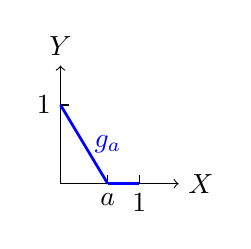
\begin{tikzpicture}
                    \coordinate (O) at (0,0);
                    \coordinate (X1) at (1,0);
                    \coordinate (Y1) at (0,1);
                    \coordinate (a) at (0.6,0);
                    \coordinate (X) at (1.5,0);
                    \coordinate (Y) at (0,1.5);
                    % ++ means adding extra distance
                    \draw (X1) node[below] {$1$} -- ++(0, 3pt);
                    \draw (a) node[below] {$a$} -- ++(0, 3pt);
                    \draw (Y1) node[left] {$1$} -- ++(3pt,0);
                    \draw[->] (O) -- (X) node[right] {$X$}; 
                    \draw[->] (O) -- (Y) node [above] {$Y$}; 
                    \draw[line width=0.35mm,color=blue] (a) -- (X1);
                    \draw[line width=0.35mm,color=blue] (Y1) -- node[right] {$g_a$} (a);
                \end{tikzpicture}
                \ \ \ \ \ \ \ \ \ \ \ \
                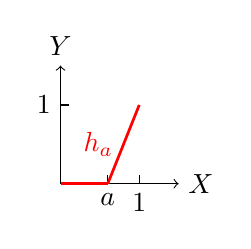
\begin{tikzpicture}
                    \coordinate (O) at (0,0);
                    \coordinate (X1) at (1,0);
                    \coordinate (Y1) at (0,1);
                    \coordinate (Y2) at (1,1);
                    \coordinate (a) at (0.6,0);
                    \coordinate (X) at (1.5,0);
                    \coordinate (Y) at (0,1.5);
                    % ++ means adding extra distance
                    \draw (X1) node[below] {$1$} -- ++(0, 3pt);
                    \draw (a) node[below] {$a$} -- ++(0, 3pt);
                    \draw (Y1) node[left] {$1$} -- ++(3pt,0);
                    \draw[->] (O) -- (X) node[right] {$X$}; 
                    \draw[->] (O) -- (Y) node [above] {$Y$}; 
                    \draw[line width=0.35mm,color=red] (O) -- (a);
                    \draw[line width=0.35mm,color=red] (a) -- node[left] {$h_a$} (Y2);
                \end{tikzpicture}
            \end{center}
        \item Claim. $\operatorname{Nil}(R) = 0$. Let $f \in \operatorname{Nil}(R)$. Then $f^{m} = 0$ for some $m \geq 1$. Then $(f(a))^{m} = 0$ for $a \in [0,1]$. Since $f([0,1]) \subseteq \bbR$ and $\bbR$ is an integral domain, $f(a) = 0$ for $a \in [0,1]$, i.e., $f= 0$.
        \item Claim. $(0:f) = \operatorname{rad}(0:f)$ for $f \in R$. ``$\subseteq$''. Done. ``$\supseteq$''. Let $g \in \operatorname{rad}(0:f)$. Then $g^{m} \cdot f = 0$ and so $g^{m}f^{m} = 0$. Then $gf \in \operatorname{Nil}(R) = 0$ by (c). So $g \in (0:f)$. 
        \item Claim. $(0:f) \not \in \operatorname{Spec}(R)$ for $f \in R$. Suppose $(0:f) \in \operatorname{Spec}(R)$. Then $(0:f) \neq R$ and so $f \neq 0$. Then there exists $y \in [0,1]$ such that $f(y) \neq 0$. Since $f$ is continuous, there exists $y \in (0,1)$ such that $f(y) \neq 0$. Let $0 < x < y$. Then $g_xh_x = 0 \in (0:f) \in \operatorname{Spec}(R)$. 
            \begin{center}
                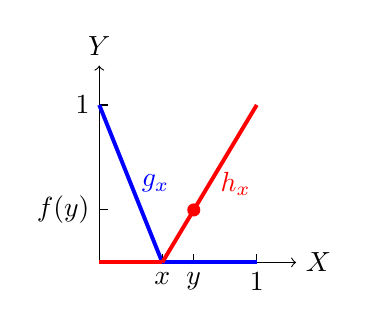
\begin{tikzpicture}
                    \coordinate (O) at (0,0);
                    \coordinate (X1) at (2,0);
                    \coordinate (Y1) at (0,2);
                    \coordinate (Y2) at (2,2);
                    \coordinate (Y3) at (1.2,0);
                    \coordinate (Y4) at (0,2/3);
                    \coordinate (a) at (0.8,0);
                    \coordinate (X) at (2.5,0);
                    \coordinate (Y) at (0,2.5);
                    % ++ means adding extra distance
                    \draw (X1) node[below] {$1$} -- ++(0, 3pt);
                    \draw (a) node[below] {$x$} -- ++(0, 3pt);
                    \draw (Y3) node[below] {$y$} -- ++(0, 3pt);
                    \draw (Y1) node[left] {$1$} -- ++(3pt,0);
                    \draw (Y4) node[left] {$f(y)$} -- ++(3pt,0);
                    \draw[->] (O) -- (X) node[right] {$X$}; 
                    \draw[->] (O) -- (Y) node [above] {$Y$}; 
                    \draw[line width=0.5mm,color = blue] (a) -- (X1);
                    \draw[line width=0.5mm,color=blue] (Y1) -- node[right] {$g_x$} (a);
                    \draw[line width=0.5mm,color = red] (O) -- (a);
                    \draw[line width=0.5mm,color=red] (a) -- node[right] {$h_x$} (Y2);
                    \draw[red,fill=red] (1.2,2/3) circle (.5ex);
                \end{tikzpicture}
            \end{center}
            So $g_x \in (0:f)$ or $h_x \in (0:f)$, i.e., $g_xf = 0$ or $h_xf =  0$. Also, since $h_x(y)f(y) > 0$, we have $h_xf \neq 0$. So $g_xf = 0$ for all $0 < x < y$. Also, since $g_x(a) \neq 0$ for $0 < a < x < y$, we have $f(a) = 0$ for $0 < a < x < y$. So $f(a) = 0$ for $0 < a < y$. Also, since $f$ is continuous, $f(y) = \lim_{a \to y^{-}}f(a) = 0$, a contradiction. \par 
            Now suppose $0 = \bigcap_{i=1}^{n}\ffq_i$ is a primary decomposition. Assume without loss of generality that the decomposition is minimal by Proposition 4.27. Note for $i = 1,\cdots,n$, there exists $f_i \in R$ such that $\operatorname{Spec}(R) \not \ni (0:f_i) = \operatorname{rad}(0:f_i) = \operatorname{rad}(\ffq_i) \in \operatorname{Spec}(R)$ by Proposition 4.30, a contradiction. 
        \item Note $0 = \bigcap_{a \in [0,1]} \ker(\Phi_a) = \bigcap_{a \in [0,1]} \smallunderbrace{\{f \in R \mid f(a) = 0\}}_{\in \operatorname{Spec}(R),\ \therefore \text{ primary}} = \bigcap_{a \in [0,1] \cap \bbQ} \ker(\Phi_a)$ cannot be pruned to a minimal decomposition.
    \end{enumerate}
\end{example}

\begin{proposition}
    If $\ffa \lneq R$ with a minimal primary decomposition $\ffa = \bigcap_{i=1}^{n} \ffq_i$ such that $\ffp_i = \operatorname{rad}(\ffq_i)$ for $i = 1,\cdots,n$, then $D := \{x \in R \mid (\ffa:x) \neq \ffa\} = \bigcup_{i=1}^{n} \ffp_i = \bigcup_{\ffp \in \operatorname{Ass}_R(\ffa)} \ffp$.
\end{proposition}

\begin{proof}
    Claim. $D = \bigcup_{y \not\in \ffa} \operatorname{rad}(\ffa:y)$. ``$\subseteq$''. Let $x \in D$. Then $x \in R$ such that $(\ffa:x) \neq \ffa$. So $(\ffa:x) \supsetneq \ffa$. Then there exists $y \in (\ffa:x) \setminus \ffa$, i.e., $y \not \in \ffa$ and $xy \in \ffa$, i.e., $y \not \in \ffa$ and $x \in (\ffa:y) \subseteq \operatorname{rad}(\ffa:y) \subseteq \bigcup_{y \not\in \ffa} \operatorname{rad}(\ffa:y)$. ``$\supseteq$''. Let $x \in \operatorname{rad}(\ffa:y)$ for some $y \in R \setminus \ffa$. Then $x^{m}y \in \ffq$ for some $m \geq 1$. Let $n = \min\{m \geq 1 \mid x^{m}y \in \ffa\}$. Note $x^{0}y = y \not \in \ffa$. Then $x^{n}y \in \ffa$ but $x^{n-1}y \not \in \ffa$. So $x^{n-1}y \in (\ffa:x)$. Hence $(\ffa:x) \neq \ffa$. Thus, $x \in D$. \par 
    Claim. $D = \bigcup_{i=1}^{n}\ffp_i$. ``$\subseteq$''. Let $y \not\in \ffa = \bigcap_{i=1}^{n} \ffq_i$. By the proof of Proposition 4.30, $\operatorname{rad}(\ffa:y) = \bigcap_{i=1,y \not \in \ffq_i}^{n} \ffp_i = \bigcap_{i=1}^{n} \ffp_i \subseteq \bigcup_{i=1}^{n}\ffp_i$. ``$\supseteq$''. By Proposition 4.30, there exists $y_i \not \in \ffa$ such that $\ffp_i = \operatorname{rad}(\ffa:y_i)$ for $i = 1,\cdots,i$. So $\bigcup_{i=1}^{n} \ffp_i \subseteq D$. 
\end{proof}

\begin{corollary}
    If $0 \lneq R$ has a mimimal primary decomposition $0 = \bigcap_{i=1}^{n} \ffq_i$ such that $\ffp_i = \operatorname{rad}(\ffq_i)$ for $i = 1,\cdots,n$, then $\operatorname{ZD}(R) = \bigcup_{i=1}^{n} \ffp_i = \bigcup_{\ffp \in \operatorname{Ass}_R(0)}\ffp$.
\end{corollary}

\begin{summary}
    Let $R$ be noetherian and $0$ has a minimal primary decomposition $0 = \bigcap_{i=1}^{n} \ffq_i$ such that $\ffp_i = \operatorname{rad}(\ffq_i)$ for $i = 1,\cdots,n$. $\operatorname{ZD}(R) = \bigcup_{i=1}^{n} \ffp_i = \bigcup_{\ffp \in \operatorname{Ass}(R)(0)}\ffp$. (Use with prime avoidence to get useful information about ideals and $\operatorname{NZD}(R)$). $\operatorname{Nil}(R) = \bigcap_{i=1}^{n} \ffp_i = \bigcap_{\ffp \in \operatorname{Min}(0)} \ffp$.
\end{summary}

\begin{example*}
    Let $R = \frac{k[X,Y]}{\langle X^{2},XY \rangle} = \frac{k[X,Y]}{\langle X \rangle \cap \langle X^{2},Y \rangle}$. Then $\langle 0 \rangle R = \langle \overbar{X} \rangle \cap \langle \overbar{X}^{2}, \overbar{Y} \rangle$ is a minimal primary decomposition. So $\operatorname{ZD}(R) = \langle \overbar{X} \rangle \cup \langle \overbar{X}, \overbar{Y} \rangle = \langle \overbar{X}, \overbar{Y} \rangle$. For $f \in R$ with constant term 0, we have $f = \overbar{X}f_1 + \overbar{Y}f_2$ for some $f_1,f_2 \in R$, then $\overbar{X}f = \overbar{X}^{2}f_1 + \overbar{X} \overbar{Y} f_2 = 0$. So $f \in \operatorname{ZD}(R)$.
\end{example*}

\begin{proposition}
    Let $\ffa \lneq R$ with a minimal primary decomposition $\ffa = \bigcap_{i=1}^{n} \ffq_i$ such that $\ffp_i = \operatorname{rad}(\ffq_i)$ for $i = 1,\cdots,n$. Then $\operatorname{Min}(\ffa) = \min\{\ffp_1,\cdots,\ffp_n\} = \min\{\operatorname{V}(\ffa)\} = \min\{\ffp \supseteq \ffa\}$. 
\end{proposition}

\begin{proof}
    By Proposition 4.28, $\operatorname{V}(\ffa) = \bigcup_{\ffp \in \operatorname{Min}(\ffa)} \operatorname{V}(\ffp)$. 
\end{proof}

\begin{lemma}
    Let $U \subseteq R$ be multiplicatively closed and $\ffq \lneq R$ be $\ffp$-primary. Let $\psi: R \to U^{-1}R$ be the natural ring homomorphism.
    \begin{enumerate}
        \item If $U \cap \ffp \neq \emptyset$, then $U^{-1}\ffq = U^{-1}R$.
        \item If $U \cap \ffp = \emptyset$, then $U^{-1}\ffq \lneq U^{-1}R$ is $U^{-1}\ffp$-primary and $\psi^{-1}(U^{-1}\ffq) = \ffq$.
    \end{enumerate}
\end{lemma}

\begin{proof}
    \begin{enumerate}
        \item Let $u \in U \cap \ffp$. Since $\ffp = \operatorname{rad}(\ffq)$ and $U$ is multiplicatively closed, there exists $n \geq 1$ such that $u^{n} \in \ffq \cap U$. So by Proposition 3.13, $U^{-1}\ffq = U^{-1}R$.
        \item Since $\ffq \subseteq \ffp$ and $U \cap \ffp = \emptyset$, $U^{-1}\ffq \subseteq U^{-1}\ffp \subsetneq U^{-1}R$ by Proposition 3.13. \par 
            Let $\frac{x}{u},\frac{y}{v} \in U^{-1}R$ such that $\frac{x}{u} \cdot \frac{y}{v} \in U^{-1}\ffq$. If $\frac{y}{v} \in \operatorname{rad}(U^{-1}\ffq)$, then done. Assume $\frac{y}{v} \not \in \operatorname{rad}(U^{-1}\ffq)$. Since $\frac{xy}{uv} \in U^{-1}\ffq$, there exists $w \in U$ such that $x(wy) = wxy \in \ffq$. Since $\frac{y}{v} \not\in \operatorname{rad}(U^{-1}\ffq) = U^{-1} \operatorname{rad}(\ffq) = U^{-1}\ffp$ by Proposition 3.12(d), $wy \not \in \ffp = \operatorname{rad}(\ffq)$. Also, since $\ffq$ is primary, $x \in \ffq$. So $\frac{x}{u} \in U^{-1}\ffq$. Hence $U^{-1}\ffq$ is primary. \par
            Since $\ffq \subseteq \ffp = \operatorname{rad}(\ffq) \in \operatorname{Spec}(R)$, by Proposition 3.12(d), we have $\operatorname{rad}(U^{-1}\ffq) \subseteq \operatorname{rad}(U^{-1}\ffp) = U^{-1} \operatorname{rad}(\ffp) = U^{-1}\ffp = U^{-1} \operatorname{rad}(\ffq) = \operatorname{rad}(U^{-1}\ffq)$. So $\operatorname{rad}(U^{-1}\ffq) = U^{-1}\ffp$. \par
            Claim. $\psi^{-1}(U^{-1}\ffq) = \ffq$. ``$\supseteq$''. By Proposition 1.63(a). ``$\subseteq$''. Let $x \in \psi^{-1}(U^{-1}\ffq)$. Then $\frac{x}{1} = \psi(x) \in U^{-1}\ffq$. So there exists $u \in U$ such that $ux \in \ffq$. Since $U \cap \ffp = \emptyset$, $u \not \in \ffp = \operatorname{rad}(\ffq)$. Also, since $\ffq$ is primary, $x \in \ffq$. \qedhere
    \end{enumerate}
\end{proof}

\begin{theorem}[Second uniqueness theorem]
    Let $\ffa \lneq R$ with a minimal primary decomposition $\ffa = \bigcap_{i=1}^{n} \ffq_i$ such that $\ffp_i = \operatorname{rad}(\ffq_i)$ for $i = 1,\cdots,n$. 
    \begin{enumerate}
        \item For $\ffp_i \in \operatorname{Min}(\ffa)$ with $i \in \{1,\cdots,n\}$: $\ffq_i = \psi^{-1}(\ffa_{\ffp_i})$, where $\psi: R \to R_{\ffp_i}$ with $U = R \setminus \ffp_i$, so $\ffq_i$ is independent of choice of minimal decomposition.
        \item If $\Lambda = \langle \ffp_{i_1},\cdots,\ffp_{i_m} \rangle$ is an ``isolated'' subset of $\operatorname{Ass}_R(\ffa) = \{\ffp_1,\cdots,\ffp_n\}$, then $\bigcap_{j=1}^{m} \ffq_{i_j} = \Psi^{-1}(U^{-1}\ffa)$, where $\Psi: R \to U^{-1}R$ and $U = R \setminus \{\ffp_{i_1} \cup \cdots \cup \ffp_{i_m}\}$. So $\bigcap_{j=1}^{m}\ffq_{i_j}$ is independent of choice of minimal decomposition.
    \end{enumerate}
\end{theorem}

\begin{proof}
    \begin{enumerate}
        \item [(b)] By Proposition 3.12(b) and Lemma 4.37, we have $\Psi^{-1}(U^{-1}\ffa) = \Psi^{-1}(U^{-1}(\bigcap_{i=1}^{n}\ffq_i)) = \Psi^{-1}(\bigcap_{i=1}^{n}U^{-1}\ffq_i) = \bigcap_{i=1}^{n} \Psi^{-1}(U^{-1}\ffq_i) = \bigcap_{i=1,\ffp_i \cap U = \emptyset}^{n} \ffq_i = \bigcap_{j=1}^{m} \ffq_{i_j}$ since $\Lambda$ is isolated.
        \item [(a)] It follows from (b) since $\{\ffp_i\}$ is isolated for $\ffp_i \in \operatorname{Min}(\ffa)$. \qedhere
    \end{enumerate}
\end{proof}

\begin{definition}
    $\Lambda \subseteq \operatorname{Ass}_R(\ffa)$ is ``isolated'' if it is ``closed under subsets'', i.e., if $\ffp_i, \ffp_j \in \operatorname{Ass}_R(\ffa)$ such that $\ffp_j \subseteq \ffp_i$ and $\ffp_i \in \Lambda$, then $\ffp_j \in \Lambda$.
\end{definition}

\begin{discussion}
    \begin{enumerate}
        \item
            If $\ffm \in \operatorname{m-Spec}(R)$, then $\ffm^{n}$ is $\ffm$-primary for $n \geq 1$ by Example 4.11(b). \par 
        \item 
            Let $k$ be a field. If $\ffp = \langle X_{i_1}, \cdots, X_{i_m} \rangle \lneq k[X_1,\cdots,X_d]$, then $\ffp^{n}$ is $\ffp$-primary for $n \geq 1$.
    \end{enumerate}
\end{discussion}

\begin{proof}
    \begin{enumerate}
        \item[(b)]
            Note $\langle X_{i_1}^{a_1},\cdots,X_{i_m}^{a_m} \rangle$ is $\ffp$-primary for $a_1,\cdots,a_m \geq 1$ by Example 4.12(c). Let $\Lambda = \{\underline a \in \bbN^{m} \mid a_1 + \cdots + a_m = m+n-1\}$. Set $\ffp_{\underline a} = \langle X_{i_1}^{a_1},\cdots,X_{i_m}^{a_m} \rangle$ for $\underline a \in \Lambda$. Claim. $\ffp^{n} = \bigcap_{\underline a \in \Lambda} \ffp_{\underline a}$, then by Proposition 4.22, $\ffp^{n}$ is $\ffp$-primary. \par
            ``$\subseteq$''. Let $\Lambda_0 = \{\underline e \in \bbZ_{\geq 0}^{m} \mid e_1 + \cdots + e_m = n\}$. For $n \geq 1$, $\ffp^{n} = (\langle X_{i_1} \rangle + \cdots + \langle X_{i_m} \rangle)^{n} = \sum_{\underline e \in \Lambda_0} \langle X_{i_1}^{e_1} \cdots X_{i_m}^{e_m} \rangle$. Suppose $X_{(i)}^{\underline e} := X_{i_1}^{e_1} \cdots X_{i_m}^{e_m} \in \ffp^{n} \setminus \ffp_{\underline a}$ for some $\underline e \in \Lambda_0$ and $\underline a \in \Lambda$. Then $a_i \geq e_i+1$ for $i = 1,\cdots,m$. So $m+n-1 = \sum_{i=1}^{m}a_i \geq m + \sum_{i=1}^{m}e_i = m+n$, a contradiction. So $X^{\underline e}_{(i)} \in \ffp_{\underline a}$ for all $\underline e \in \Lambda_0$ and $\underline a \in \Lambda$. Hence $\ffp^{n} \subseteq \bigcap_{\underline a \in \Lambda} \ffp_{\underline a}$. \par 
            ``$\supseteq$''. Let $R' := k[X_{i_1},\cdots,X_{i_m}] \subseteq k[X_1,\cdots,X_d]$ and $\ffp' = (X_{i_1},\cdots,X_{i_m})R'$. Set $\ffp'_{\underline a} = \langle X_{i_1}^{a_1},\cdots,X_{i_m}^{a_m} \rangle R'$ for $\underline a \in \Lambda$. We know $\ffp'^{n}$ in $R'$ has a (irredundant) parametric decomposition $\ffp'^{n} = \bigcap_{f \text{ is a $\ffp'$-corner element in $R'$}} P_R(f) = \bigcap_{\underline a \in \Lambda} \ffp'_{\underline a}$. Let $q = \# \Lambda$. Since $\bigcap_{\underline a \in \Lambda} \ffp_{\underline a}$ and $\bigcap_{\underline a \in \Lambda} \ffp'_{\underline a}$ have the same generating set $\{\operatorname{lcm}(f_1,\cdots,f_q) \mid f_j \text{ is a generator of $\ffp_{\underline a_j}$ with $\underline a_j \in \Lambda$ for $j=1,\cdots,q$}\}$, we have the generators of $\bigcap_{\underline a \in \Lambda} \ffp_{\underline a}$ are in $\bigcap_{\underline a \in \Lambda} \ffp_{\underline a}' = \ffp'^{n} \subseteq \ffp^{n}$. Hence $\ffp^{n} \supseteq \bigcap_{\underline a \in \Lambda} \ffp_{\underline a}$. \qedhere
    \end{enumerate}
\end{proof}

\begin{example}
    In general, $\ffp^{n}$ is not $\ffp$-primary for $\ffp \in \operatorname{Spec}(R)$. For example, let $R = \frac{k[X,Y,Z]}{\langle XY-Z^{2} \rangle}$ and $x := \overline x,y := \overline Y, z := \overline Z \in R$, then $\ffp := \langle x,z \rangle \in \operatorname{Spec}(R)$, but $\ffp^{2}$ is not $\ffp$-primary since $xy = z^{2} \in \ffp^{2}$ but $x \not \in \ffp^{2}$ and $y \not \in \ffp = \operatorname{rad}(\ffp^{2})$.
\end{example}

\begin{definition}
Let $\ffp \in \operatorname{Spec}(R)$ and $\psi: R \to R_\ffp$. Then for $n \geq 1$, the $n^{th}$ \emph{symbolic power} of $\ffp$ is $\ffp^{(n)} = \psi^{-1}((\ffp^{n})_\ffp) = \psi^{-1}\left( \ffp_\ffp \right)^{n})$. 
\end{definition}

\begin{note}
    $\ffp^{n} \subseteq \ffp^{(n)}$ because by Proposition 1.63(a), $\ffp^{n} \subseteq \psi^{-1}((\ffp^{n})_\ffp) = \ffp^{(n)}$.
\end{note}

\begin{example}
    \begin{enumerate}
        \item 
            Let $\ffm \in \operatorname{m-Spec}(R)$ and $\psi: R \to R_\ffm$. Since $\ffm^{n}$ is $\ffm$-primary by Example 4.11(b) and $\ffm \cap (R \setminus \ffm) = \emptyset$, by Lemma 4.37(b), $\ffm^{n} = \psi^{-1}((\ffm^{n})_\ffm) =: \ffm^{(n)}$ for $n \geq 1$. 
        \item Let $k$ be a field and $\ffp = \langle X_{i_1}, \cdots, X_{i_m} \rangle \lneq k[X_1,\cdots,X_d]$. Since $\ffp^{n}$ is $\ffp$-primary by Discussion 4.40(b) and $\ffp \cap (R \setminus \ffp) = \emptyset$, by Lemma 4.37(b), $\ffp^{n} = \psi^{-1}((\ffp^{n})_\ffp) =: \ffp^{(n)}$ for $n \geq 1$.
        \item Let $R = \frac{k[X,Y,Z]}{\langle XY-Z^{2} \rangle}$ and $x = \overbar X, y = \overline Y, z = \overbar Z \in R$. Let $\ffp = \langle x, z \rangle$. Claim $\ffp^{(2)} = \langle x \rangle$. ``$\supseteq$''. Since $y \not \in \ffp$ and $xy = z^{2} \in \ffp^{2}$, we have $x = \frac{x}{1} = \frac{xy}{y} \in (\ffp^{2})_\ffp$ in $R_\ffp$. So $x \in \psi^{-1}(\ffp^{2})_\ffp) = \ffp^{(2)}$. ``$\subseteq$''. ... Let $a \in \ffp^{(n)}$. Then $\frac{a}{1} = \psi(a) \in (\ffp^{2})_\ffp$. So there exists $b \in R \setminus \ffp$ such that $ab \in \ffp^{2} = \langle x^{2},xz,z^{2} \rangle = \langle x^{2}, xz,xy \rangle$. Also, since $b \not \in \langle x \rangle$, $a \in \langle x \rangle$. Hence $\ffp^{(2)} = \langle x \rangle \supsetneq \langle x^{2},xz,xy \rangle = \langle x^{2},xz,z^{2} \rangle = \ffp^{2}$.
    \end{enumerate}
\end{example}

\begin{proposition}
    If $\ffp \in \operatorname{Spec}(R)$, then $\ffp^{(n)}$ is the ``$\ffp$-primary component'' of $\ffp^{n}$, i.e., if $\ffp^{n}$ has a minimal primary decomposition $\ffp^{n} = \bigcap_{i=1}^{m} \ffq_i$ such that $\ffp_i = \operatorname{rad}(\ffq_i)$ for $i = 1,\cdots,m$, then $\ffp_j = \ffp$ and $\ffq_j = \ffp^{(n)}$ for some $j \in \{1,\cdots,m\}$. 
\end{proposition}

\begin{proof}
    Since $\operatorname{rad}(\ffp^{n}) = \ffp$, $\operatorname{Min}(\ffp^{n}) = \{\ffp\}$. So $\ffp = \operatorname{rad}(\ffq_i) = \ffp_i$ for some $i \in \{1,\cdots,m\}$. By Second uniqueness theorem, $\ffq_i = \psi^{-1}((\ffp_i^{n})_{\ffp_i}) = \psi^{-1}((\ffp^{n})_\ffp) = \ffp^{(n)}$.
\end{proof}

\begin{example}
    Let $R = \frac{k[X,Y,Z]}{\langle XY-Z^{2} \rangle}$ and $x = \overbar{X}, y = \overbar{Y}, z = \overbar{Z} \in R$. Let $\ffp = \langle x,z \rangle \in \operatorname{Spec}(R)$. Then by Example 4.44(c), $\ffp^{(2)} = \langle x \rangle$. Note $\ffp^{2} = \langle x \rangle \cap \langle x^{2},z,y \rangle$. Since $z^{2} = xy \in \langle x \rangle$, $\operatorname{rad}(\langle x \rangle) = \langle x,z \rangle$. Since $R/\langle x,y,z \rangle \cong \frac{k[X,Y,X]}{\langle XY-Z^{2},X,Y,Z \rangle} = \frac{k[X,Y,Z]}{\langle X,Y,Z \rangle} \cong k$, $\operatorname{rad}(\langle x^{2},z,y \rangle) = \langle x,y,z \rangle \in \operatorname{m-Spec}(R)$.
\end{example}

\begin{definition}[Calculus content]
\end{definition}
